% The LaTeX is in here!
\documentclass[12pt]{article}
\renewcommand{\baselinestretch}{1.5} 
\usepackage{graphicx}
\usepackage{ragged2e}
\usepackage{parskip}
\usepackage{float}
\fontfamily{Arial}\selectfont
\renewcommand{\familydefault}{\sfdefault}
\usepackage{listings}
\newcommand{\code}[1]{\texttt{#1}}
\usepackage{hyperref}
\usepackage[utf8]{inputenc}
\setlength{\parindent}{4em}
\usepackage[english]{babel}
\usepackage{geometry}
  \geometry{
    a4paper,
    total={170mm,257mm},
    left=30mm,
    right=30mm,
    top=20mm,
  }
\graphicspath{ {images/} }

\begin{document}
    \begin{center}
    
\includegraphics[scale=0.5]{unb}
    \par
    \vspace{15mm}
    \normalsize{Universidade de Brasília - UnB}\\
    \normalsize{Instituto de Exatas}\\
    \normalsize{Departamento de Ciência da Computação}\\
    \vspace{15mm}
    \normalsize{Rodrigo Chaves - 13/0132624}\\
    \normalsize{Gabriel Mesquita - 13/0024242}\\
    \vspace{15mm}
    \Huge{Test-drive Development}\\

    \vspace{60mm}
    \normalsize{Brasília - DF}\\
    \textnormal{2016}
  \end{center}

  \clearpage

  \begin{center}
    Gabriel Mesquita ...\\
    Rodrigo de Araujo Chaves\\
    \vspace{30mm}
    \Huge{Test-driven Development}
    \vspace{30mm}
    \normalsize{}
    \begin{flushright}
      Dissertação sobre por que Test-driven development\\
      é pratica que melhorar a qualidade\\
      final do software apresentanda à disciplina\\
      de Engenharia de Software da Universidade de Brasília.\\
    \end{flushright}
  \end{center}

  \clearpage

  \section{Introdução}

  Hoje, no Brasil, não há dados confiáveis sobre quantos reais são perdidos por
  software defeituosos, mas especialistas afirmam que 8 bilhões de reais é um
  valor bem próximo da realidade brasileira. Um exemplo que pode demonstrar o 
  prejuízo de um software mal fabricado pode causar foi a sonda espacial Mars 
  Climate Orbiter, perdida na atmosfera de Marte por errar a unidade em um
  cálculo, misturando as medidas de pés e metros.

  Apesar desses danos de falhas serem custosos quando o software é colocado em
  produção, essas falhas também podem causar dor de cabeça as desenvolvedores e
  todos os stakeholders envolvidos durante a fase de desenvolvimento.

  \section{O que é Test-driven Development}

  Test-driven development é um prática de desenvolvimento de software que tem 
  sido usada esporádicamente por decadas. Com essa prática, um engenheiro de 
  software passo por ciclos entre escrever um teste de unidade que falha e 
  escrevendo a implementação do software para passar nesses testes. 
  Test-driven development tem recentemente resurgindo como uma pratica critica 
  possibilitando metodologias de desenvolvimento ágil de software.

  Quando discutimos sobre TDD, é considerado um conjunto de tarefas requiridas 
  que podem ser implementadas em poucos dias ou menos. Na imagem 1, engenheiros 
  de software produzem código de produção através de rápidas interações como as 
  que seguem:

  \begin{enumerate}
    \item O primeiro passo é adicionar um teste simples o qual é suficiente 
    para a suíte de teste falhar.
    \item Depois executamos nossa suíte para confirmar que os testes realmente 
    estão falhando.
    \item Agora atualize-se o código funcional afim de passar no novo teste.
    \item Executamos a suíte de teste para verificarmos se agora realmente 
    passarmos no novo teste.
    \item Agora com o teste passando: são removidos as duplicações de código 
    afim de limpar o código.
  \end{enumerate}

  \begin{figure}[H]
    \centering
    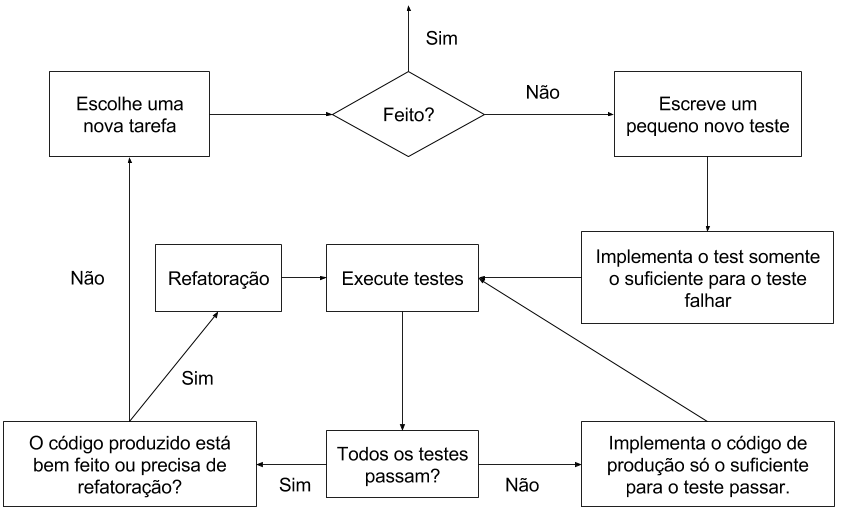
\includegraphics[scale=0.4]{tdd}
    \caption{Fluxograma do TDD}
  \end{figure}

  \section{Automação de Testes}

  No desenvolvimento orientado à Testes, uma ferramenta muito imporantante são
  os frameworks de testes automatizados para a criação de objetos orientados
  a testes de unidade. 

  Em Ruby, por exemplo, o framework \code{RSpec} é comumente usado onde cada Classe 
  Pública tem um class correspondente \code{<NomeDaClasse>TestCase}. Para cada
  método público dessa classe, é criado um \code{test<NomeDoMétodo>} onde o 
  contrato do método é testado. Além disso, outros \code{test<NomeDoMétodo>}s 
  são criados para validar o comportamento desse método com diferentes 
  parametros. A cada execução de um \code{test<NomeDoMétodo>}, um método 
  \code{setUP} é chamado e esse é responsável por criar as variáveis de teste,
  criar a instância de \code{<NomeDaClasse>} e executar o respectivo método.
  No final, um método \code{tearDown} é chamado para resetar as variáveis.

  Uma prática comum do usos do framework de automação de testes é usar cores
  para expressar o resultados da suíte de testes. Caso algum teste não passe,
  a cor vermelha é usada para indicar a atenção do desenvolvedor. Caso todos os
  testes passem, usamos a cor verde para indicar os resultados dos testes. A 
  imagem a baixo demonstra de forma simplificada qual é o ritmo comum dentro do
  ciclo do Test-driven Development.

  \begin{figure}[H]
    \centering
    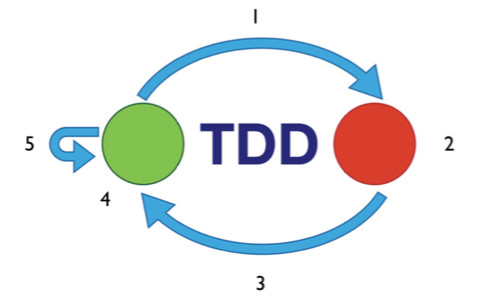
\includegraphics[scale=1.0]{tdd_micro}
    \caption{Colograma do TDD}
  \end{figure}

  \section{Design de Software em TDD}

  O Test-driven Development permite que o desenvolvedor que está trabalhando 
  em um módulo pense como serão as responsabilidades, interfaces, serviços os 
  quais serão disponibilizados por esse módulo, enquanto escreve os testes. 
  Depois, quando vai escrever o código de produção, pode se preocupar somente em
  implementar o necessário para passar nos teste já feitos. Fazendo assim, 
  criamos um ritmo entre codificação e teste até que todos os testes criados 
  sejam implementados.

  Pensando no design do projeto, os desenvolvedores do projeto podem criar
  classes e módulos mais coesoes e menos acopladas por que, durante a fase de 
  elaboração dos testes, conseguem visualizar a arquitetura geral da aplicação e
  melhorar como o compenente que irão desenvolver irá conservar com os outros 
  componentes. Em alguns testes, os desenvolvedores os escrevem usando o 
  componente em desenvolvimento como já estivesse pronto e validam se
  esse consegue ser comunicar com suas interfaces.

  Em Test-driven Development, o código desenvolvido é mantido dentro do controle
  intelectual do desenvolvedor, já que o próprio escreveu os testes e ele ou 
  ela está fazendo continuadamente pequenas alterações de design e decisões de 
  implementação, aumentando as funcionalidades do programa em um certo ritmo 
  contínuo.

  \section{Desenvolvimento Ágil e Test-driven Development}

  Test-driven development é uma prática sugerida dentro do "Extremming 
  Programming", também muito conhecido por XP, por Kent Beck. XP é surgiu nos
  Estados Unidos e tem ganhado bastante espaço no desenvolvimento de software
  pois é um conjunto de valores, principios e práticas que fazem os softwares 
  serem produzidos em menos tempo e de forma mais econômica que o habitual.

  Desenvolvimento incremental é uma prática que não só traz benefícios. Ao se
  adicionar novas funcionalidade a um software, há um risco de falhas serem 
  introduzidas. O XP adotou o usou de Test-driven Development como um mecanismo
  de proteção impedindo que algo que já estivesse funcionando fosse quebrado
  e não detectado. “O desenvolvimento orientado a testes é uma forma de lidar 
  com o medo durante a programação (BECK, 2003).”

  Os testes automatizados criados pelos desenvolvedores formam uma base de 
  testes que pode ser executada sempre que necessário visualizar se tudo está
  funcionando normalmente. Isso não impede que falhas sejam inseridas, porém
  é uma forma detecção possibilitando uma correção efetiva e barata, impedindo
  que bugs se acumulem com o passar do tempo.

  \section{Objetivos ao se praticar TDD}

  TDD é uma prática de desenvolvimento que tem por objetivo garantir a
  qualidade e a confiabilidade do produto o mais rápido possível. Ao decorrer do
  desenvolvimento, todo o código elaborado é desenvolvido em conjunto com uma
  suíte de testes automatizados. Esses testes permitem uma segurança maior ao
  desenvolvedor quando precisa mudar algo que já foi implementado ou precisa 
  refotaror o código.

  Além disso, desenvolvedores experientes em TDD podem analisar se os testes 
  produzidos estão difíceis de serem feitos e podem fazer refactoring ou 
  mudanças.

  \section{Depuração}

  Quando é detectado um defeito em um software, é necessário consertá-lo. Nesse
  momento, entramos na fase de depuração. Se observamos os programadores 
  realizando suas atividades, iremos perceber que eles levam mais tempo é 
  depurando. Uma pequena parte é feita a codificação propriamente dita. O 
  restante do tempo é gasto projetando-se e entendo o que deve ser feito.

  Consertar a falha identificada é fácil, porém encontrar onde está acontecendo
  o problema é o que leva a fase de depuração ser tão longa. As equipes de 
  desenvolvimento podem usar o Test-driven Development para serem capazes de
  identificar mais rápidamente essas falhas.

  Além disso, ao se consertar um falha local, existe uma possibilidade (entre
  20 a 50 por cento) de se introduzir uma nova falha. As bases de testes 
  automatizados facilitam a garantir que as correções feitas não introduzem 
  novos problemas pois conseguem testar as outras funcionalidades do sistema
  ao ser executada.

  \section{Referências}

  \begin{flushleft}
  Nachiappan Nagappan, E. Michael Maximilien, Thirumalesh Bhat,
  Laurie Williams, Realizing quality improvement through test driven 
  development: results and experiences of four industrial teams. Disponível em
  \url{http://link.springer.com/article/10.1007/s10664-008-9062-z#/page-1}.
  Acessado em 26 de maio de 2016.

  Andreas Augustin, Test-Driven Development: Concepts, Taxonomy, and Future 
  Direction. Disponível em \url{https://www.semanticscholar.org/paper/Test-
  Driven-Development-Concepts-Taxonomy-and-Janzen-Saiedian/bdcd570eb6a45d7a
  9107a18e25f54b741b92177f/pdf}. Acessado em 26 de maio de 2016

  Martin Fowler, Bill Venners: Test-Driven Development, A Conversation with 
  Martin Fowler. Disponível em \url{http://www.biology.emory.edu/research/Prinz
  /Cengiz/cs540-485-FA12/resources/testDrivenDev.pdf}. Acessado em 30 de maio de
  2016.

  Mauricio Finavaro Aniche, Como a prática de TDD influencia o projeto de 
  classes em sistemas orientados a objetos. Disponível em 
  \url{http://www.teses.usp.br/teses/disponiveis/45/45134/tde-31072012-181230
  /publico/dissertacao.pdf}. Acessado em 30 de maio de 2016.

  Roger Pressman, Software Engineering: A Practitioner’s Approach, 7/e 
  (McGraw-Hill, 2009), capítulo 3.  Disponível em
  \url{http://academic.brooklyn.cuny.edu/cis/sfleisher/Chapter_03_sim.pdf}.
  Acessado em 1º de junho de 2016.

  Vínicius Manhães Teles, Um estudo de caso da adoção das práticas e valores do
  extremme programming. Disponível em
  \url{http://www.improveit.com.br/xp/dissertacaoXP.pdf}. Acessado em 1º de 
  junho de 2016.

  Laurie Williams, E. Michael Maximilien, Mladen Vouk, Test-Driven Development 
  as a Defect-Reduction Practice. Disponível em 
  \url{ftp://www.ufv.br/dpi/mestrado/TDD
  /willians_TDD_Defect-Reducion_Practice.pdf}. Acessado em 1º de Junho de 2016.

  André Faria Gomes, Agile, Desenvolvimento de Software com entregas frequentes
  e foco no valor de negócio. Casa do Código.
  
  \end{flushleft}

\end{document}